\documentclass[1p]{elsarticle_modified}
%\bibliographystyle{elsarticle-num}

%\usepackage[colorlinks]{hyperref}
%\usepackage{abbrmath_seonhwa} %\Abb, \Ascr, \Acal ,\Abf, \Afrak
\usepackage{amsfonts}
\usepackage{amssymb}
\usepackage{amsmath}
\usepackage{amsthm}
\usepackage{scalefnt}
\usepackage{amsbsy}
\usepackage{kotex}
\usepackage{caption}
\usepackage{subfig}
\usepackage{color}
\usepackage{graphicx}
\usepackage{xcolor} %% white, black, red, green, blue, cyan, magenta, yellow
\usepackage{float}
\usepackage{setspace}
\usepackage{hyperref}

\usepackage{tikz}
\usetikzlibrary{arrows}

\usepackage{multirow}
\usepackage{array} % fixed length table
\usepackage{hhline}

%%%%%%%%%%%%%%%%%%%%%
\makeatletter
\renewcommand*\env@matrix[1][\arraystretch]{%
	\edef\arraystretch{#1}%
	\hskip -\arraycolsep
	\let\@ifnextchar\new@ifnextchar
	\array{*\c@MaxMatrixCols c}}
\makeatother %https://tex.stackexchange.com/questions/14071/how-can-i-increase-the-line-spacing-in-a-matrix
%%%%%%%%%%%%%%%

\usepackage[normalem]{ulem}

\newcommand{\msout}[1]{\ifmmode\text{\sout{\ensuremath{#1}}}\else\sout{#1}\fi}
%SOURCE: \msout is \stkout macro in https://tex.stackexchange.com/questions/20609/strikeout-in-math-mode

\newcommand{\cancel}[1]{
	\ifmmode
	{\color{red}\msout{#1}}
	\else
	{\color{red}\sout{#1}}
	\fi
}

\newcommand{\add}[1]{
	{\color{blue}\uwave{#1}}
}

\newcommand{\replace}[2]{
	\ifmmode
	{\color{red}\msout{#1}}{\color{blue}\uwave{#2}}
	\else
	{\color{red}\sout{#1}}{\color{blue}\uwave{#2}}
	\fi
}

\newcommand{\Sol}{\mathcal{S}} %segment
\newcommand{\D}{D} %diagram
\newcommand{\A}{\mathcal{A}} %arc


%%%%%%%%%%%%%%%%%%%%%%%%%%%%%5 test

\def\sl{\operatorname{\textup{SL}}(2,\Cbb)}
\def\psl{\operatorname{\textup{PSL}}(2,\Cbb)}
\def\quan{\mkern 1mu \triangleright \mkern 1mu}

\theoremstyle{definition}
\newtheorem{thm}{Theorem}[section]
\newtheorem{prop}[thm]{Proposition}
\newtheorem{lem}[thm]{Lemma}
\newtheorem{ques}[thm]{Question}
\newtheorem{cor}[thm]{Corollary}
\newtheorem{defn}[thm]{Definition}
\newtheorem{exam}[thm]{Example}
\newtheorem{rmk}[thm]{Remark}
\newtheorem{alg}[thm]{Algorithm}

\newcommand{\I}{\sqrt{-1}}
\begin{document}

%\begin{frontmatter}
%
%\title{Boundary parabolic representations of knots up to 8 crossings}
%
%%% Group authors per affiliation:
%\author{Yunhi Cho} 
%\address{Department of Mathematics, University of Seoul, Seoul, Korea}
%\ead{yhcho@uos.ac.kr}
%
%
%\author{Seonhwa Kim} %\fnref{s_kim}}
%\address{Center for Geometry and Physics, Institute for Basic Science, Pohang, 37673, Korea}
%\ead{ryeona17@ibs.re.kr}
%
%\author{Hyuk Kim}
%\address{Department of Mathematical Sciences, Seoul National University, Seoul 08826, Korea}
%\ead{hyukkim@snu.ac.kr}
%
%\author{Seokbeom Yoon}
%\address{Department of Mathematical Sciences, Seoul National University, Seoul, 08826,  Korea}
%\ead{sbyoon15@snu.ac.kr}
%
%\begin{abstract}
%We find all boundary parabolic representation of knots up to 8 crossings.
%
%\end{abstract}
%\begin{keyword}
%    \MSC[2010] 57M25 
%\end{keyword}
%
%\end{frontmatter}

%\linenumbers
%\tableofcontents
%
\newcommand\colored[1]{\textcolor{white}{\rule[-0.35ex]{0.8em}{1.4ex}}\kern-0.8em\color{red} #1}%
%\newcommand\colored[1]{\textcolor{white}{ #1}\kern-2.17ex	\textcolor{white}{ #1}\kern-1.81ex	\textcolor{white}{ #1}\kern-2.15ex\color{red}#1	}

{\Large $\underline{11a_{99}~(K11a_{99})}$}

\setlength{\tabcolsep}{10pt}
\renewcommand{\arraystretch}{1.6}
\vspace{1cm}\begin{tabular}{m{100pt}>{\centering\arraybackslash}m{274pt}}
\multirow{5}{120pt}{
	\centering
	\includegraphics[width=112pt]{../../../GIT/diagram.site/Diagrams/png/348_11a_99.png}\\
\ \ \ A knot diagram\footnotemark}&
\allowdisplaybreaks
\textbf{Linearized knot diagam} \\
\cline{2-2}
 &
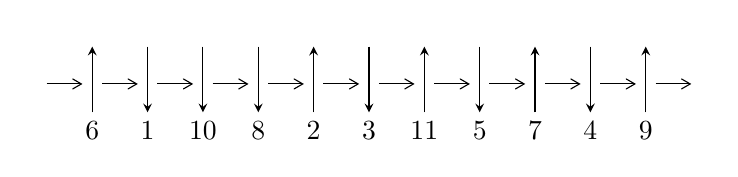
\begin{tikzpicture}[x=20pt, y=17pt]
	% nodes
	\node (C0) at (0, 0) {};
	\node (C1) at (1, 0) {};
	\node (C1U) at (1, +1) {};
	\node (C1D) at (1, -1) {6};

	\node (C2) at (2, 0) {};
	\node (C2U) at (2, +1) {};
	\node (C2D) at (2, -1) {1};

	\node (C3) at (3, 0) {};
	\node (C3U) at (3, +1) {};
	\node (C3D) at (3, -1) {10};

	\node (C4) at (4, 0) {};
	\node (C4U) at (4, +1) {};
	\node (C4D) at (4, -1) {8};

	\node (C5) at (5, 0) {};
	\node (C5U) at (5, +1) {};
	\node (C5D) at (5, -1) {2};

	\node (C6) at (6, 0) {};
	\node (C6U) at (6, +1) {};
	\node (C6D) at (6, -1) {3};

	\node (C7) at (7, 0) {};
	\node (C7U) at (7, +1) {};
	\node (C7D) at (7, -1) {11};

	\node (C8) at (8, 0) {};
	\node (C8U) at (8, +1) {};
	\node (C8D) at (8, -1) {5};

	\node (C9) at (9, 0) {};
	\node (C9U) at (9, +1) {};
	\node (C9D) at (9, -1) {7};

	\node (C10) at (10, 0) {};
	\node (C10U) at (10, +1) {};
	\node (C10D) at (10, -1) {4};

	\node (C11) at (11, 0) {};
	\node (C11U) at (11, +1) {};
	\node (C11D) at (11, -1) {9};
	\node (C12) at (12, 0) {};

	% arrows
	\draw[->,>={angle 60}]
	(C0) edge (C1) (C1) edge (C2) (C2) edge (C3) (C3) edge (C4) (C4) edge (C5) (C5) edge (C6) (C6) edge (C7) (C7) edge (C8) (C8) edge (C9) (C9) edge (C10) (C10) edge (C11) (C11) edge (C12) ;	\draw[->,>=stealth]
	(C1D) edge (C1U) (C2U) edge (C2D) (C3U) edge (C3D) (C4U) edge (C4D) (C5D) edge (C5U) (C6U) edge (C6D) (C7D) edge (C7U) (C8U) edge (C8D) (C9D) edge (C9U) (C10U) edge (C10D) (C11D) edge (C11U) ;
	\end{tikzpicture} \\
\hhline{~~} \\& 
\textbf{Solving Sequence} \\ \cline{2-2} 
 &
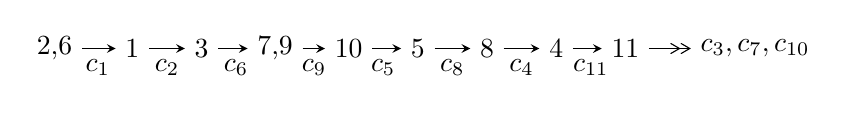
\begin{tikzpicture}[x=25pt, y=7pt]
	% node
	\node (A0) at (-1/8, 0) {2,6};
	\node (A1) at (1, 0) {1};
	\node (A2) at (2, 0) {3};
	\node (A3) at (49/16, 0) {7,9};
	\node (A4) at (33/8, 0) {10};
	\node (A5) at (41/8, 0) {5};
	\node (A6) at (49/8, 0) {8};
	\node (A7) at (57/8, 0) {4};
	\node (A8) at (65/8, 0) {11};
	\node (C1) at (1/2, -1) {$c_{1}$};
	\node (C2) at (3/2, -1) {$c_{2}$};
	\node (C3) at (5/2, -1) {$c_{6}$};
	\node (C4) at (29/8, -1) {$c_{9}$};
	\node (C5) at (37/8, -1) {$c_{5}$};
	\node (C6) at (45/8, -1) {$c_{8}$};
	\node (C7) at (53/8, -1) {$c_{4}$};
	\node (C8) at (61/8, -1) {$c_{11}$};
	\node (A9) at (10, 0) {$c_{3},c_{7},c_{10}$};

	% edge
	\draw[->,>=stealth]	
	(A0) edge (A1) (A1) edge (A2) (A2) edge (A3) (A3) edge (A4) (A4) edge (A5) (A5) edge (A6) (A6) edge (A7) (A7) edge (A8) ;
	\draw[->>,>={angle 60}]	
	(A8) edge (A9);
\end{tikzpicture} \\ 

\end{tabular} \\

\footnotetext{
The image of knot diagram is generated by the software ``\textbf{Draw programme}" developed by Andrew Bartholomew(\url{http://www.layer8.co.uk/maths/draw/index.htm\#Running-draw}), where we modified some parts for our purpose(\url{https://github.com/CATsTAILs/LinksPainter}).
}\phantom \\ \newline 
\centering \textbf{Ideals for irreducible components\footnotemark of $X_{\text{par}}$} 
 
\begin{align*}
I^u_{1}&=\langle 
-3 u^{27}-26 u^{26}+\cdots+2 b-6,\;9 u^{27}+72 u^{26}+\cdots+4 a+84,\;u^{28}+6 u^{27}+\cdots+26 u+4\rangle \\
I^u_{2}&=\langle 
5947395 u^9 a^3-110563267 u^9 a^2+\cdots+261341462 a-88347236,\;- u^9 a^3-5 u^9 a^2+\cdots-8 a-7,\\
\phantom{I^u_{2}}&\phantom{= \langle  }u^{10}- u^9+3 u^8-3 u^7+5 u^6-5 u^5+4 u^4-4 u^3+3 u^2-2 u+1\rangle \\
I^u_{3}&=\langle 
u^{11}- u^{10}+4 u^9-3 u^8+7 u^7-4 u^6+4 u^5- u^3+3 u^2+b-2 u+3,\\
\phantom{I^u_{3}}&\phantom{= \langle  }-2 u^{12}+u^{11}-6 u^{10}+u^9-8 u^8- u^7-2 u^6-4 u^5+u^4-2 u^3+a-2 u-2,\\
\phantom{I^u_{3}}&\phantom{= \langle  }u^{13}- u^{12}+4 u^{11}-3 u^{10}+7 u^9-4 u^8+5 u^7- u^6+2 u^4-2 u^3+3 u^2- u+1\rangle \\
I^u_{4}&=\langle 
a^3 u- a^2 u^2+a^2 u+u^2 a- a^2+4 u^2+b+a-2 u+5,\\
\phantom{I^u_{4}}&\phantom{= \langle  }a^4-3 a^2 u^2+a^3+3 a^2 u-3 u^2 a-4 a^2+3 a u+9 u^2-4 a-6 u+13,\;u^3+u+1\rangle \\
\\
\end{align*}
\raggedright * 4 irreducible components of $\dim_{\mathbb{C}}=0$, with total 93 representations.\\
\footnotetext{All coefficients of polynomials are rational numbers. But the coefficients are sometimes approximated in decimal forms when there is not enough margin.}
\newpage
\renewcommand{\arraystretch}{1}
\centering \section*{I. $I^u_{1}= \langle -3 u^{27}-26 u^{26}+\cdots+2 b-6,\;9 u^{27}+72 u^{26}+\cdots+4 a+84,\;u^{28}+6 u^{27}+\cdots+26 u+4 \rangle$}
\flushleft \textbf{(i) Arc colorings}\\
\begin{tabular}{m{7pt} m{180pt} m{7pt} m{180pt} }
\flushright $a_{2}=$&$\begin{pmatrix}1\\0\end{pmatrix}$ \\
\flushright $a_{6}=$&$\begin{pmatrix}0\\u\end{pmatrix}$ \\
\flushright $a_{1}=$&$\begin{pmatrix}1\\u^2\end{pmatrix}$ \\
\flushright $a_{3}=$&$\begin{pmatrix}u^2+1\\u^4\end{pmatrix}$ \\
\flushright $a_{7}=$&$\begin{pmatrix}- u^5-2 u^3- u\\- u^7- u^5+u\end{pmatrix}$ \\
\flushright $a_{9}=$&$\begin{pmatrix}-\frac{9}{4} u^{27}-18 u^{26}+\cdots-\frac{513}{4} u-21\\\frac{3}{2} u^{27}+13 u^{26}+\cdots+\frac{77}{2} u+3\end{pmatrix}$ \\
\flushright $a_{10}=$&$\begin{pmatrix}\frac{11}{4} u^{27}+14 u^{26}+\cdots+\frac{143}{4} u+5\\-\frac{5}{2} u^{27}-15 u^{26}+\cdots-\frac{127}{2} u-11\end{pmatrix}$ \\
\flushright $a_{5}=$&$\begin{pmatrix}- u\\u\end{pmatrix}$ \\
\flushright $a_{8}=$&$\begin{pmatrix}-\frac{21}{4} u^{27}-29 u^{26}+\cdots-\frac{449}{4} u-19\\\frac{9}{2} u^{27}+24 u^{26}+\cdots+\frac{45}{2} u+1\end{pmatrix}$ \\
\flushright $a_{4}=$&$\begin{pmatrix}-\frac{1}{2} u^{27}-\frac{3}{2} u^{26}+\cdots-\frac{41}{2} u-\frac{7}{2}\\-\frac{5}{2} u^{27}-14 u^{26}+\cdots-\frac{55}{2} u-4\end{pmatrix}$ \\
\flushright $a_{11}=$&$\begin{pmatrix}\frac{1}{2} u^{27}+\frac{9}{2} u^{26}+\cdots+\frac{73}{2} u+\frac{13}{2}\\-\frac{1}{2} u^{27}-3 u^{26}+\cdots+\frac{7}{2} u+2\end{pmatrix}$\\ \flushright $a_{11}=$&$\begin{pmatrix}\frac{1}{2} u^{27}+\frac{9}{2} u^{26}+\cdots+\frac{73}{2} u+\frac{13}{2}\\-\frac{1}{2} u^{27}-3 u^{26}+\cdots+\frac{7}{2} u+2\end{pmatrix}$\\&\end{tabular}
\flushleft \textbf{(ii) Obstruction class $= -1$}\\~\\
\flushleft \textbf{(iii) Cusp Shapes $= -13 u^{27}-78 u^{26}-316 u^{25}-906 u^{24}-2126 u^{23}-4197 u^{22}-7359 u^{21}-11710 u^{20}-17291 u^{19}-23878 u^{18}-30954 u^{17}-37835 u^{16}-43786 u^{15}-48249 u^{14}-50700 u^{13}-50669 u^{12}-48099 u^{11}-43213 u^{10}-36755 u^9-29326 u^8-21691 u^7-14716 u^6-9106 u^5-5172 u^4-2641 u^3-1112 u^2-342 u-54$}\\~\\
\newpage\renewcommand{\arraystretch}{1}
\flushleft \textbf{(iv) u-Polynomials at the component}\newline \\
\begin{tabular}{m{50pt}|m{274pt}}
Crossings & \hspace{64pt}u-Polynomials at each crossing \\
\hline $$\begin{aligned}c_{1},c_{5}\end{aligned}$$&$\begin{aligned}
&u^{28}-6 u^{27}+\cdots-26 u+4
\end{aligned}$\\
\hline $$\begin{aligned}c_{2}\end{aligned}$$&$\begin{aligned}
&u^{28}+14 u^{27}+\cdots+36 u+16
\end{aligned}$\\
\hline $$\begin{aligned}c_{3},c_{4},c_{8}\\c_{10}\end{aligned}$$&$\begin{aligned}
&u^{28}+u^{27}+\cdots+3 u+1
\end{aligned}$\\
\hline $$\begin{aligned}c_{6}\end{aligned}$$&$\begin{aligned}
&u^{28}+6 u^{27}+\cdots+1800 u+712
\end{aligned}$\\
\hline $$\begin{aligned}c_{7}\end{aligned}$$&$\begin{aligned}
&u^{28}-29 u^{27}+\cdots-118784 u+8192
\end{aligned}$\\
\hline $$\begin{aligned}c_{9},c_{11}\end{aligned}$$&$\begin{aligned}
&u^{28}-2 u^{27}+\cdots-2 u+1
\end{aligned}$\\
\hline
\end{tabular}\\~\\
\newpage\renewcommand{\arraystretch}{1}
\flushleft \textbf{(v) Riley Polynomials at the component}\newline \\
\begin{tabular}{m{50pt}|m{274pt}}
Crossings & \hspace{64pt}Riley Polynomials at each crossing \\
\hline $$\begin{aligned}c_{1},c_{5}\end{aligned}$$&$\begin{aligned}
&y^{28}+14 y^{27}+\cdots+36 y+16
\end{aligned}$\\
\hline $$\begin{aligned}c_{2}\end{aligned}$$&$\begin{aligned}
&y^{28}-2 y^{27}+\cdots-240 y+256
\end{aligned}$\\
\hline $$\begin{aligned}c_{3},c_{4},c_{8}\\c_{10}\end{aligned}$$&$\begin{aligned}
&y^{28}-23 y^{27}+\cdots+3 y+1
\end{aligned}$\\
\hline $$\begin{aligned}c_{6}\end{aligned}$$&$\begin{aligned}
&y^{28}-18 y^{27}+\cdots+1943360 y+506944
\end{aligned}$\\
\hline $$\begin{aligned}c_{7}\end{aligned}$$&$\begin{aligned}
&y^{28}+3 y^{27}+\cdots+486539264 y+67108864
\end{aligned}$\\
\hline $$\begin{aligned}c_{9},c_{11}\end{aligned}$$&$\begin{aligned}
&y^{28}+6 y^{27}+\cdots+40 y+1
\end{aligned}$\\
\hline
\end{tabular}\\~\\
\newpage\flushleft \textbf{(vi) Complex Volumes and Cusp Shapes}
$$\begin{array}{c|c|c}  
\text{Solutions to }I^u_{1}& \I (\text{vol} + \sqrt{-1}CS) & \text{Cusp shape}\\
 \hline 
\begin{aligned}
u &= -1.007890 + 0.244456 I \\
a &= \phantom{-}0.648218 + 0.649776 I \\
b &= \phantom{-}0.484897 - 0.362346 I\end{aligned}
 & -5.75558 + 1.16478 I & -9.81484 - 5.25007 I \\ \hline\begin{aligned}
u &= -1.007890 - 0.244456 I \\
a &= \phantom{-}0.648218 - 0.649776 I \\
b &= \phantom{-}0.484897 + 0.362346 I\end{aligned}
 & -5.75558 - 1.16478 I & -9.81484 + 5.25007 I \\ \hline\begin{aligned}
u &= \phantom{-}0.450069 + 0.945327 I \\
a &= \phantom{-}0.97063 - 1.16479 I \\
b &= -0.92359 + 1.77022 I\end{aligned}
 & \phantom{-}1.30775 + 2.44749 I & -4.69640 - 9.53101 I \\ \hline\begin{aligned}
u &= \phantom{-}0.450069 - 0.945327 I \\
a &= \phantom{-}0.97063 + 1.16479 I \\
b &= -0.92359 - 1.77022 I\end{aligned}
 & \phantom{-}1.30775 - 2.44749 I & -4.69640 + 9.53101 I \\ \hline\begin{aligned}
u &= \phantom{-}0.823545 + 0.669603 I \\
a &= -0.244511 + 1.089610 I \\
b &= -0.807023 - 0.636285 I\end{aligned}
 & -2.90686 - 3.71581 I & -3.96472 + 7.21162 I \\ \hline\begin{aligned}
u &= \phantom{-}0.823545 - 0.669603 I \\
a &= -0.244511 - 1.089610 I \\
b &= -0.807023 + 0.636285 I\end{aligned}
 & -2.90686 + 3.71581 I & -3.96472 - 7.21162 I \\ \hline\begin{aligned}
u &= -0.877743 + 0.205256 I \\
a &= -1.36751 - 0.95489 I \\
b &= -0.332382 + 1.109600 I\end{aligned}
 & -7.91511 + 11.38140 I & -4.44423 - 5.90932 I \\ \hline\begin{aligned}
u &= -0.877743 - 0.205256 I \\
a &= -1.36751 + 0.95489 I \\
b &= -0.332382 - 1.109600 I\end{aligned}
 & -7.91511 - 11.38140 I & -4.44423 + 5.90932 I \\ \hline\begin{aligned}
u &= \phantom{-}0.693563 + 0.915180 I \\
a &= -1.289000 - 0.358838 I \\
b &= \phantom{-}1.64479 - 0.73716 I\end{aligned}
 & -3.67868 + 9.29135 I & -4.02619 - 9.42557 I \\ \hline\begin{aligned}
u &= \phantom{-}0.693563 - 0.915180 I \\
a &= -1.289000 + 0.358838 I \\
b &= \phantom{-}1.64479 + 0.73716 I\end{aligned}
 & -3.67868 - 9.29135 I & -4.02619 + 9.42557 I\\
 \hline 
 \end{array}$$\newpage$$\begin{array}{c|c|c}  
\text{Solutions to }I^u_{1}& \I (\text{vol} + \sqrt{-1}CS) & \text{Cusp shape}\\
 \hline 
\begin{aligned}
u &= -0.417630 + 1.105260 I \\
a &= -0.990060 - 0.503261 I \\
b &= \phantom{-}0.343945 + 0.624215 I\end{aligned}
 & -2.12382 - 1.70105 I & -2.95787 + 0.05705 I \\ \hline\begin{aligned}
u &= -0.417630 - 1.105260 I \\
a &= -0.990060 + 0.503261 I \\
b &= \phantom{-}0.343945 - 0.624215 I\end{aligned}
 & -2.12382 + 1.70105 I & -2.95787 - 0.05705 I \\ \hline\begin{aligned}
u &= -0.483475 + 1.130610 I \\
a &= \phantom{-}1.03565 + 1.24896 I \\
b &= -0.38060 - 1.45896 I\end{aligned}
 & -1.61917 - 5.94948 I & -1.73292 + 6.08838 I \\ \hline\begin{aligned}
u &= -0.483475 - 1.130610 I \\
a &= \phantom{-}1.03565 - 1.24896 I \\
b &= -0.38060 + 1.45896 I\end{aligned}
 & -1.61917 + 5.94948 I & -1.73292 - 6.08838 I \\ \hline\begin{aligned}
u &= \phantom{-}0.433444 + 0.634083 I \\
a &= \phantom{-}1.80511 - 0.76581 I \\
b &= -1.031200 + 0.788265 I\end{aligned}
 & \phantom{-}2.24308 + 1.31021 I & \phantom{-}4.48172 + 2.40271 I \\ \hline\begin{aligned}
u &= \phantom{-}0.433444 - 0.634083 I \\
a &= \phantom{-}1.80511 + 0.76581 I \\
b &= -1.031200 - 0.788265 I\end{aligned}
 & \phantom{-}2.24308 - 1.31021 I & \phantom{-}4.48172 - 2.40271 I \\ \hline\begin{aligned}
u &= -0.305330 + 0.675911 I \\
a &= -0.630555 + 0.172210 I \\
b &= \phantom{-}0.360299 + 0.412592 I\end{aligned}
 & -0.257625 - 1.154960 I & -2.96071 + 5.77634 I \\ \hline\begin{aligned}
u &= -0.305330 - 0.675911 I \\
a &= -0.630555 - 0.172210 I \\
b &= \phantom{-}0.360299 - 0.412592 I\end{aligned}
 & -0.257625 + 1.154960 I & -2.96071 - 5.77634 I \\ \hline\begin{aligned}
u &= -0.315106 + 1.262770 I \\
a &= \phantom{-}0.488001 + 0.002907 I \\
b &= \phantom{-}0.100408 + 1.021430 I\end{aligned}
 & -12.6068 + 7.4137 I & -9.32623 - 3.45211 I \\ \hline\begin{aligned}
u &= -0.315106 - 1.262770 I \\
a &= \phantom{-}0.488001 - 0.002907 I \\
b &= \phantom{-}0.100408 - 1.021430 I\end{aligned}
 & -12.6068 - 7.4137 I & -9.32623 + 3.45211 I\\
 \hline 
 \end{array}$$\newpage$$\begin{array}{c|c|c}  
\text{Solutions to }I^u_{1}& \I (\text{vol} + \sqrt{-1}CS) & \text{Cusp shape}\\
 \hline 
\begin{aligned}
u &= -0.554721 + 1.203480 I \\
a &= -1.83799 - 0.92930 I \\
b &= \phantom{-}1.96223 + 2.11484 I\end{aligned}
 & -10.9151 - 16.6086 I & -7.19926 + 9.00617 I \\ \hline\begin{aligned}
u &= -0.554721 - 1.203480 I \\
a &= -1.83799 + 0.92930 I \\
b &= \phantom{-}1.96223 - 2.11484 I\end{aligned}
 & -10.9151 + 16.6086 I & -7.19926 - 9.00617 I \\ \hline\begin{aligned}
u &= -0.243939 + 1.326510 I \\
a &= -0.0674133 + 0.0418679 I \\
b &= -0.033141 - 1.007620 I\end{aligned}
 & -11.26130 - 3.02152 I & -13.62827 + 2.14467 I \\ \hline\begin{aligned}
u &= -0.243939 - 1.326510 I \\
a &= -0.0674133 - 0.0418679 I \\
b &= -0.033141 + 1.007620 I\end{aligned}
 & -11.26130 + 3.02152 I & -13.62827 - 2.14467 I \\ \hline\begin{aligned}
u &= -0.608424 + 0.177740 I \\
a &= \phantom{-}0.665110 - 0.192137 I \\
b &= -0.474963 - 0.907755 I\end{aligned}
 & \phantom{-}1.04620 + 1.66789 I & \phantom{-}3.14449 - 2.66380 I \\ \hline\begin{aligned}
u &= -0.608424 - 0.177740 I \\
a &= \phantom{-}0.665110 + 0.192137 I \\
b &= -0.474963 + 0.907755 I\end{aligned}
 & \phantom{-}1.04620 - 1.66789 I & \phantom{-}3.14449 + 2.66380 I \\ \hline\begin{aligned}
u &= -0.586363 + 1.242360 I \\
a &= \phantom{-}1.064320 + 0.381059 I \\
b &= -1.41368 - 1.21973 I\end{aligned}
 & -8.88695 - 6.88314 I & -9.37455 + 6.80974 I \\ \hline\begin{aligned}
u &= -0.586363 - 1.242360 I \\
a &= \phantom{-}1.064320 - 0.381059 I \\
b &= -1.41368 + 1.21973 I\end{aligned}
 & -8.88695 + 6.88314 I & -9.37455 - 6.80974 I\\
 \hline 
 \end{array}$$\newpage\newpage\renewcommand{\arraystretch}{1}
\centering \section*{II. $I^u_{2}= \langle 5.95\times10^{6} a^{3} u^{9}-1.11\times10^{8} a^{2} u^{9}+\cdots+2.61\times10^{8} a-8.83\times10^{7},\;- u^9 a^3-5 u^9 a^2+\cdots-8 a-7,\;u^{10}- u^9+\cdots-2 u+1 \rangle$}
\flushleft \textbf{(i) Arc colorings}\\
\begin{tabular}{m{7pt} m{180pt} m{7pt} m{180pt} }
\flushright $a_{2}=$&$\begin{pmatrix}1\\0\end{pmatrix}$ \\
\flushright $a_{6}=$&$\begin{pmatrix}0\\u\end{pmatrix}$ \\
\flushright $a_{1}=$&$\begin{pmatrix}1\\u^2\end{pmatrix}$ \\
\flushright $a_{3}=$&$\begin{pmatrix}u^2+1\\u^4\end{pmatrix}$ \\
\flushright $a_{7}=$&$\begin{pmatrix}- u^5-2 u^3- u\\- u^7- u^5+u\end{pmatrix}$ \\
\flushright $a_{9}=$&$\begin{pmatrix}a\\-0.0456620 a^{3} u^{9}+0.848865 a^{2} u^{9}+\cdots-2.00649 a+0.678298\end{pmatrix}$ \\
\flushright $a_{10}=$&$\begin{pmatrix}2.14382 a^{3} u^{9}+1.09367 a^{2} u^{9}+\cdots-1.51933 a+0.196840\\-0.260987 a^{3} u^{9}+0.338504 a^{2} u^{9}+\cdots+0.870243 a+2.69447\end{pmatrix}$ \\
\flushright $a_{5}=$&$\begin{pmatrix}- u\\u\end{pmatrix}$ \\
\flushright $a_{8}=$&$\begin{pmatrix}0.0644237 a^{3} u^{9}+0.101106 a^{2} u^{9}+\cdots-1.19004 a-1.96492\\-0.110086 a^{3} u^{9}+0.747759 a^{2} u^{9}+\cdots+0.183553 a+2.64322\end{pmatrix}$ \\
\flushright $a_{4}=$&$\begin{pmatrix}-0.770676 a^{3} u^{9}-0.285432 a^{2} u^{9}+\cdots-0.188169 a-1.85717\\-0.0386232 a^{3} u^{9}+0.223455 a^{2} u^{9}+\cdots+1.74875 a+3.11581\end{pmatrix}$ \\
\flushright $a_{11}=$&$\begin{pmatrix}-0.277440 a^{3} u^{9}-0.327129 a^{2} u^{9}+\cdots-0.0644294 a+0.411808\\-0.285316 a^{3} u^{9}+0.175678 a^{2} u^{9}+\cdots+0.268957 a-0.519132\end{pmatrix}$\\ \flushright $a_{11}=$&$\begin{pmatrix}-0.277440 a^{3} u^{9}-0.327129 a^{2} u^{9}+\cdots-0.0644294 a+0.411808\\-0.285316 a^{3} u^{9}+0.175678 a^{2} u^{9}+\cdots+0.268957 a-0.519132\end{pmatrix}$\\&\end{tabular}
\flushleft \textbf{(ii) Obstruction class $= -1$}\\~\\
\flushleft \textbf{(iii) Cusp Shapes $= \frac{6098888}{7661669} u^9 a^3-\frac{21091308}{7661669} u^9 a^2+\cdots+\frac{116819364}{7661669} a+\frac{59639590}{7661669}$}\\~\\
\newpage\renewcommand{\arraystretch}{1}
\flushleft \textbf{(iv) u-Polynomials at the component}\newline \\
\begin{tabular}{m{50pt}|m{274pt}}
Crossings & \hspace{64pt}u-Polynomials at each crossing \\
\hline $$\begin{aligned}c_{1},c_{5}\end{aligned}$$&$\begin{aligned}
&(u^{10}+u^9+3 u^8+3 u^7+5 u^6+5 u^5+4 u^4+4 u^3+3 u^2+2 u+1)^4
\end{aligned}$\\
\hline $$\begin{aligned}c_{2}\end{aligned}$$&$\begin{aligned}
&(u^{10}+5 u^9+13 u^8+19 u^7+17 u^6+7 u^5-2 u^3+u^2+2 u+1)^4
\end{aligned}$\\
\hline $$\begin{aligned}c_{3},c_{4},c_{8}\\c_{10}\end{aligned}$$&$\begin{aligned}
&u^{40}- u^{39}+\cdots-18 u^2+1
\end{aligned}$\\
\hline $$\begin{aligned}c_{6}\end{aligned}$$&$\begin{aligned}
&(u^{10}+2 u^9- u^8-5 u^7-3 u^6+4 u^5+12 u^4+13 u^3+5 u^2+u+2)^4
\end{aligned}$\\
\hline $$\begin{aligned}c_{7}\end{aligned}$$&$\begin{aligned}
&(u^2+u+1)^{20}
\end{aligned}$\\
\hline $$\begin{aligned}c_{9},c_{11}\end{aligned}$$&$\begin{aligned}
&u^{40}+11 u^{39}+\cdots+644 u+61
\end{aligned}$\\
\hline
\end{tabular}\\~\\
\newpage\renewcommand{\arraystretch}{1}
\flushleft \textbf{(v) Riley Polynomials at the component}\newline \\
\begin{tabular}{m{50pt}|m{274pt}}
Crossings & \hspace{64pt}Riley Polynomials at each crossing \\
\hline $$\begin{aligned}c_{1},c_{5}\end{aligned}$$&$\begin{aligned}
&(y^{10}+5 y^9+13 y^8+19 y^7+17 y^6+7 y^5-2 y^3+y^2+2 y+1)^4
\end{aligned}$\\
\hline $$\begin{aligned}c_{2}\end{aligned}$$&$\begin{aligned}
&(y^{10}+y^9+13 y^8+11 y^7+45 y^6+35 y^5+12 y^4+2 y^3+9 y^2-2 y+1)^4
\end{aligned}$\\
\hline $$\begin{aligned}c_{3},c_{4},c_{8}\\c_{10}\end{aligned}$$&$\begin{aligned}
&y^{40}-33 y^{39}+\cdots-36 y+1
\end{aligned}$\\
\hline $$\begin{aligned}c_{6}\end{aligned}$$&$\begin{aligned}
&(y^{10}-6 y^9+\cdots+19 y+4)^{4}
\end{aligned}$\\
\hline $$\begin{aligned}c_{7}\end{aligned}$$&$\begin{aligned}
&(y^2+y+1)^{20}
\end{aligned}$\\
\hline $$\begin{aligned}c_{9},c_{11}\end{aligned}$$&$\begin{aligned}
&y^{40}+11 y^{39}+\cdots+62528 y+3721
\end{aligned}$\\
\hline
\end{tabular}\\~\\
\newpage\flushleft \textbf{(vi) Complex Volumes and Cusp Shapes}
$$\begin{array}{c|c|c}  
\text{Solutions to }I^u_{2}& \I (\text{vol} + \sqrt{-1}CS) & \text{Cusp shape}\\
 \hline 
\begin{aligned}
u &= -0.584958 + 0.771492 I \\
a &= -0.811252 - 0.684607 I \\
b &= \phantom{-}0.326566 + 1.346250 I\end{aligned}
 & \phantom{-}0.002387 - 0.280172 I & -1.136314 + 0.057227 I \\ \hline\begin{aligned}
u &= -0.584958 + 0.771492 I \\
a &= -0.13825 + 1.48131 I \\
b &= \phantom{-}0.856552 - 0.765235 I\end{aligned}
 & \phantom{-}0.002387 - 0.280172 I & -1.136314 + 0.057227 I \\ \hline\begin{aligned}
u &= -0.584958 + 0.771492 I \\
a &= \phantom{-}1.41803 - 0.77086 I \\
b &= -1.87810 - 0.26325 I\end{aligned}
 & \phantom{-}0.00239 - 4.33994 I & -1.13631 + 6.98543 I \\ \hline\begin{aligned}
u &= -0.584958 + 0.771492 I \\
a &= -1.63324 - 0.44978 I \\
b &= \phantom{-}0.783367 + 0.997354 I\end{aligned}
 & \phantom{-}0.00239 - 4.33994 I & -1.13631 + 6.98543 I \\ \hline\begin{aligned}
u &= -0.584958 - 0.771492 I \\
a &= -0.811252 + 0.684607 I \\
b &= \phantom{-}0.326566 - 1.346250 I\end{aligned}
 & \phantom{-}0.002387 + 0.280172 I & -1.136314 - 0.057227 I \\ \hline\begin{aligned}
u &= -0.584958 - 0.771492 I \\
a &= -0.13825 - 1.48131 I \\
b &= \phantom{-}0.856552 + 0.765235 I\end{aligned}
 & \phantom{-}0.002387 + 0.280172 I & -1.136314 - 0.057227 I \\ \hline\begin{aligned}
u &= -0.584958 - 0.771492 I \\
a &= \phantom{-}1.41803 + 0.77086 I \\
b &= -1.87810 + 0.26325 I\end{aligned}
 & \phantom{-}0.00239 + 4.33994 I & -1.13631 - 6.98543 I \\ \hline\begin{aligned}
u &= -0.584958 - 0.771492 I \\
a &= -1.63324 + 0.44978 I \\
b &= \phantom{-}0.783367 - 0.997354 I\end{aligned}
 & \phantom{-}0.00239 + 4.33994 I & -1.13631 - 6.98543 I \\ \hline\begin{aligned}
u &= \phantom{-}0.248527 + 0.782547 I \\
a &= -0.528657 + 0.220233 I \\
b &= \phantom{-}0.80276 - 1.85708 I\end{aligned}
 & -5.38286 + 3.26157 I & -6.90177 - 8.91318 I \\ \hline\begin{aligned}
u &= \phantom{-}0.248527 + 0.782547 I \\
a &= -0.77879 + 1.65055 I \\
b &= -0.1103870 - 0.0163537 I\end{aligned}
 & -5.38286 - 0.79819 I & -6.90177 - 1.98497 I\\
 \hline 
 \end{array}$$\newpage$$\begin{array}{c|c|c}  
\text{Solutions to }I^u_{2}& \I (\text{vol} + \sqrt{-1}CS) & \text{Cusp shape}\\
 \hline 
\begin{aligned}
u &= \phantom{-}0.248527 + 0.782547 I \\
a &= -2.16490 - 1.33388 I \\
b &= \phantom{-}2.78977 + 0.25266 I\end{aligned}
 & -5.38286 - 0.79819 I & -6.90177 - 1.98497 I \\ \hline\begin{aligned}
u &= \phantom{-}0.248527 + 0.782547 I \\
a &= \phantom{-}2.27476 + 2.17074 I \\
b &= -1.93781 - 0.58149 I\end{aligned}
 & -5.38286 + 3.26157 I & -6.90177 - 8.91318 I \\ \hline\begin{aligned}
u &= \phantom{-}0.248527 - 0.782547 I \\
a &= -0.528657 - 0.220233 I \\
b &= \phantom{-}0.80276 + 1.85708 I\end{aligned}
 & -5.38286 - 3.26157 I & -6.90177 + 8.91318 I \\ \hline\begin{aligned}
u &= \phantom{-}0.248527 - 0.782547 I \\
a &= -0.77879 - 1.65055 I \\
b &= -0.1103870 + 0.0163537 I\end{aligned}
 & -5.38286 + 0.79819 I & -6.90177 + 1.98497 I \\ \hline\begin{aligned}
u &= \phantom{-}0.248527 - 0.782547 I \\
a &= -2.16490 + 1.33388 I \\
b &= \phantom{-}2.78977 - 0.25266 I\end{aligned}
 & -5.38286 + 0.79819 I & -6.90177 + 1.98497 I \\ \hline\begin{aligned}
u &= \phantom{-}0.248527 - 0.782547 I \\
a &= \phantom{-}2.27476 - 2.17074 I \\
b &= -1.93781 + 0.58149 I\end{aligned}
 & -5.38286 - 3.26157 I & -6.90177 + 8.91318 I \\ \hline\begin{aligned}
u &= \phantom{-}0.761643 + 0.208049 I \\
a &= -0.888121 - 0.198095 I \\
b &= \phantom{-}0.169145 - 1.209710 I\end{aligned}
 & -2.52120 - 5.50828 I & -2.80497 + 6.25925 I \\ \hline\begin{aligned}
u &= \phantom{-}0.761643 + 0.208049 I \\
a &= -1.109160 + 0.691872 I \\
b &= -0.405801 - 0.684900 I\end{aligned}
 & -2.52120 - 1.44851 I & -2.80497 - 0.66896 I \\ \hline\begin{aligned}
u &= \phantom{-}0.761643 + 0.208049 I \\
a &= -0.465789 - 0.420142 I \\
b &= \phantom{-}0.307020 + 0.341147 I\end{aligned}
 & -2.52120 - 1.44851 I & -2.80497 - 0.66896 I \\ \hline\begin{aligned}
u &= \phantom{-}0.761643 + 0.208049 I \\
a &= \phantom{-}1.44027 - 1.30172 I \\
b &= \phantom{-}0.177943 + 1.296040 I\end{aligned}
 & -2.52120 - 5.50828 I & -2.80497 + 6.25925 I\\
 \hline 
 \end{array}$$\newpage$$\begin{array}{c|c|c}  
\text{Solutions to }I^u_{2}& \I (\text{vol} + \sqrt{-1}CS) & \text{Cusp shape}\\
 \hline 
\begin{aligned}
u &= \phantom{-}0.761643 - 0.208049 I \\
a &= -0.888121 + 0.198095 I \\
b &= \phantom{-}0.169145 + 1.209710 I\end{aligned}
 & -2.52120 + 5.50828 I & -2.80497 - 6.25925 I \\ \hline\begin{aligned}
u &= \phantom{-}0.761643 - 0.208049 I \\
a &= -1.109160 - 0.691872 I \\
b &= -0.405801 + 0.684900 I\end{aligned}
 & -2.52120 + 1.44851 I & -2.80497 + 0.66896 I \\ \hline\begin{aligned}
u &= \phantom{-}0.761643 - 0.208049 I \\
a &= -0.465789 + 0.420142 I \\
b &= \phantom{-}0.307020 - 0.341147 I\end{aligned}
 & -2.52120 + 1.44851 I & -2.80497 + 0.66896 I \\ \hline\begin{aligned}
u &= \phantom{-}0.761643 - 0.208049 I \\
a &= \phantom{-}1.44027 + 1.30172 I \\
b &= \phantom{-}0.177943 - 1.296040 I\end{aligned}
 & -2.52120 + 5.50828 I & -2.80497 - 6.25925 I \\ \hline\begin{aligned}
u &= -0.449566 + 1.164790 I \\
a &= \phantom{-}0.79423 - 1.18245 I \\
b &= -0.42710 + 2.17011 I\end{aligned}
 & -9.81146 - 6.17573 I & -10.98134 + 7.44010 I \\ \hline\begin{aligned}
u &= -0.449566 + 1.164790 I \\
a &= \phantom{-}0.152868 - 0.428323 I \\
b &= -1.107140 - 0.677603 I\end{aligned}
 & -9.81146 - 2.11597 I & -10.98134 + 0.51190 I \\ \hline\begin{aligned}
u &= -0.449566 + 1.164790 I \\
a &= \phantom{-}1.92707 + 0.90418 I \\
b &= -1.82941 - 2.34062 I\end{aligned}
 & -9.81146 - 6.17573 I & -10.98134 + 7.44010 I \\ \hline\begin{aligned}
u &= -0.449566 + 1.164790 I \\
a &= -1.75450 - 1.78926 I \\
b &= \phantom{-}2.08774 + 2.71705 I\end{aligned}
 & -9.81146 - 2.11597 I & -10.98134 + 0.51190 I \\ \hline\begin{aligned}
u &= -0.449566 - 1.164790 I \\
a &= \phantom{-}0.79423 + 1.18245 I \\
b &= -0.42710 - 2.17011 I\end{aligned}
 & -9.81146 + 6.17573 I & -10.98134 - 7.44010 I \\ \hline\begin{aligned}
u &= -0.449566 - 1.164790 I \\
a &= \phantom{-}0.152868 + 0.428323 I \\
b &= -1.107140 + 0.677603 I\end{aligned}
 & -9.81146 + 2.11597 I & -10.98134 - 0.51190 I\\
 \hline 
 \end{array}$$\newpage$$\begin{array}{c|c|c}  
\text{Solutions to }I^u_{2}& \I (\text{vol} + \sqrt{-1}CS) & \text{Cusp shape}\\
 \hline 
\begin{aligned}
u &= -0.449566 - 1.164790 I \\
a &= \phantom{-}1.92707 - 0.90418 I \\
b &= -1.82941 + 2.34062 I\end{aligned}
 & -9.81146 + 6.17573 I & -10.98134 - 7.44010 I \\ \hline\begin{aligned}
u &= -0.449566 - 1.164790 I \\
a &= -1.75450 + 1.78926 I \\
b &= \phantom{-}2.08774 - 2.71705 I\end{aligned}
 & -9.81146 + 2.11597 I & -10.98134 - 0.51190 I \\ \hline\begin{aligned}
u &= \phantom{-}0.524355 + 1.163410 I \\
a &= \phantom{-}0.740427 + 0.151085 I \\
b &= -0.650836 - 0.191721 I\end{aligned}
 & -5.31595 + 6.25643 I & -6.17560 - 2.68471 I \\ \hline\begin{aligned}
u &= \phantom{-}0.524355 + 1.163410 I \\
a &= -1.43496 + 0.55642 I \\
b &= \phantom{-}1.51204 - 1.58158 I\end{aligned}
 & -5.31595 + 6.25643 I & -6.17560 - 2.68471 I \\ \hline\begin{aligned}
u &= \phantom{-}0.524355 + 1.163410 I \\
a &= -1.20657 + 1.25082 I \\
b &= \phantom{-}0.33739 - 1.88156 I\end{aligned}
 & -5.31595 + 10.31620 I & -6.17560 - 9.61291 I \\ \hline\begin{aligned}
u &= \phantom{-}0.524355 + 1.163410 I \\
a &= \phantom{-}2.16655 - 1.00309 I \\
b &= -2.30372 + 2.02238 I\end{aligned}
 & -5.31595 + 10.31620 I & -6.17560 - 9.61291 I \\ \hline\begin{aligned}
u &= \phantom{-}0.524355 - 1.163410 I \\
a &= \phantom{-}0.740427 - 0.151085 I \\
b &= -0.650836 + 0.191721 I\end{aligned}
 & -5.31595 - 6.25643 I & -6.17560 + 2.68471 I \\ \hline\begin{aligned}
u &= \phantom{-}0.524355 - 1.163410 I \\
a &= -1.43496 - 0.55642 I \\
b &= \phantom{-}1.51204 + 1.58158 I\end{aligned}
 & -5.31595 - 6.25643 I & -6.17560 + 2.68471 I \\ \hline\begin{aligned}
u &= \phantom{-}0.524355 - 1.163410 I \\
a &= -1.20657 - 1.25082 I \\
b &= \phantom{-}0.33739 + 1.88156 I\end{aligned}
 & -5.31595 - 10.31620 I & -6.17560 + 9.61291 I \\ \hline\begin{aligned}
u &= \phantom{-}0.524355 - 1.163410 I \\
a &= \phantom{-}2.16655 + 1.00309 I \\
b &= -2.30372 - 2.02238 I\end{aligned}
 & -5.31595 - 10.31620 I & -6.17560 + 9.61291 I\\
 \hline 
 \end{array}$$\newpage\newpage\renewcommand{\arraystretch}{1}
\centering \section*{III. $I^u_{3}= \langle u^{11}- u^{10}+\cdots+b+3,\;-2 u^{12}+u^{11}+\cdots+a-2,\;u^{13}- u^{12}+\cdots- u+1 \rangle$}
\flushleft \textbf{(i) Arc colorings}\\
\begin{tabular}{m{7pt} m{180pt} m{7pt} m{180pt} }
\flushright $a_{2}=$&$\begin{pmatrix}1\\0\end{pmatrix}$ \\
\flushright $a_{6}=$&$\begin{pmatrix}0\\u\end{pmatrix}$ \\
\flushright $a_{1}=$&$\begin{pmatrix}1\\u^2\end{pmatrix}$ \\
\flushright $a_{3}=$&$\begin{pmatrix}u^2+1\\u^4\end{pmatrix}$ \\
\flushright $a_{7}=$&$\begin{pmatrix}- u^5-2 u^3- u\\- u^7- u^5+u\end{pmatrix}$ \\
\flushright $a_{9}=$&$\begin{pmatrix}2 u^{12}- u^{11}+6 u^{10}- u^9+8 u^8+u^7+2 u^6+4 u^5- u^4+2 u^3+2 u+2\\- u^{11}+u^{10}-4 u^9+3 u^8-7 u^7+4 u^6-4 u^5+u^3-3 u^2+2 u-3\end{pmatrix}$ \\
\flushright $a_{10}=$&$\begin{pmatrix}2 u^{12}- u^{11}+6 u^{10}-2 u^9+8 u^8- u^7+2 u^6+2 u^5- u^4+2 u^3+2 u+2\\- u^{11}+u^{10}-3 u^9+3 u^8-5 u^7+4 u^6-2 u^5+u^3-2 u^2+2 u-2\end{pmatrix}$ \\
\flushright $a_{5}=$&$\begin{pmatrix}- u\\u\end{pmatrix}$ \\
\flushright $a_{8}=$&$\begin{pmatrix}u^{12}+3 u^{10}+u^9+4 u^8+3 u^7+u^6+3 u^5+u^2+2\\u^{12}-2 u^{11}+\cdots+4 u-3\end{pmatrix}$ \\
\flushright $a_{4}=$&$\begin{pmatrix}- u^{12}- u^{11}-2 u^{10}-4 u^9-2 u^8-6 u^7-3 u^5- u^4+u^3-2 u^2-3\\-2 u^{12}+3 u^{11}+\cdots-5 u+3\end{pmatrix}$ \\
\flushright $a_{11}=$&$\begin{pmatrix}u^{12}-2 u^{11}+\cdots+3 u-2\\-2 u^{12}+2 u^{11}+\cdots-4 u+1\end{pmatrix}$\\ \flushright $a_{11}=$&$\begin{pmatrix}u^{12}-2 u^{11}+\cdots+3 u-2\\-2 u^{12}+2 u^{11}+\cdots-4 u+1\end{pmatrix}$\\&\end{tabular}
\flushleft \textbf{(ii) Obstruction class $= 1$}\\~\\
\flushleft \textbf{(iii) Cusp Shapes $= 2 u^{10}-4 u^9+6 u^8-8 u^7+7 u^6-5 u^5+u^4+6 u^3-3 u^2+3 u-9$}\\~\\
\newpage\renewcommand{\arraystretch}{1}
\flushleft \textbf{(iv) u-Polynomials at the component}\newline \\
\begin{tabular}{m{50pt}|m{274pt}}
Crossings & \hspace{64pt}u-Polynomials at each crossing \\
\hline $$\begin{aligned}c_{1}\end{aligned}$$&$\begin{aligned}
&u^{13}- u^{12}+\cdots- u+1
\end{aligned}$\\
\hline $$\begin{aligned}c_{2}\end{aligned}$$&$\begin{aligned}
&u^{13}+7 u^{12}+\cdots-5 u-1
\end{aligned}$\\
\hline $$\begin{aligned}c_{3},c_{8}\end{aligned}$$&$\begin{aligned}
&u^{13}- u^{12}+\cdots+3 u+1
\end{aligned}$\\
\hline $$\begin{aligned}c_{4},c_{10}\end{aligned}$$&$\begin{aligned}
&u^{13}+u^{12}+\cdots+3 u-1
\end{aligned}$\\
\hline $$\begin{aligned}c_{5}\end{aligned}$$&$\begin{aligned}
&u^{13}+u^{12}+\cdots- u-1
\end{aligned}$\\
\hline $$\begin{aligned}c_{6}\end{aligned}$$&$\begin{aligned}
&u^{13}- u^{12}+\cdots+u-1
\end{aligned}$\\
\hline $$\begin{aligned}c_{7}\end{aligned}$$&$\begin{aligned}
&u^{13}-2 u^{12}+\cdots+2 u-1
\end{aligned}$\\
\hline $$\begin{aligned}c_{9},c_{11}\end{aligned}$$&$\begin{aligned}
&u^{13}+2 u^{12}+\cdots+2 u+1
\end{aligned}$\\
\hline
\end{tabular}\\~\\
\newpage\renewcommand{\arraystretch}{1}
\flushleft \textbf{(v) Riley Polynomials at the component}\newline \\
\begin{tabular}{m{50pt}|m{274pt}}
Crossings & \hspace{64pt}Riley Polynomials at each crossing \\
\hline $$\begin{aligned}c_{1},c_{5}\end{aligned}$$&$\begin{aligned}
&y^{13}+7 y^{12}+\cdots-5 y-1
\end{aligned}$\\
\hline $$\begin{aligned}c_{2}\end{aligned}$$&$\begin{aligned}
&y^{13}- y^{12}+\cdots+7 y-1
\end{aligned}$\\
\hline $$\begin{aligned}c_{3},c_{4},c_{8}\\c_{10}\end{aligned}$$&$\begin{aligned}
&y^{13}-15 y^{12}+\cdots-9 y-1
\end{aligned}$\\
\hline $$\begin{aligned}c_{6}\end{aligned}$$&$\begin{aligned}
&y^{13}-9 y^{12}+\cdots-11 y-1
\end{aligned}$\\
\hline $$\begin{aligned}c_{7}\end{aligned}$$&$\begin{aligned}
&y^{13}+2 y^{12}+\cdots-2 y-1
\end{aligned}$\\
\hline $$\begin{aligned}c_{9},c_{11}\end{aligned}$$&$\begin{aligned}
&y^{13}+2 y^{12}+\cdots-2 y-1
\end{aligned}$\\
\hline
\end{tabular}\\~\\
\newpage\flushleft \textbf{(vi) Complex Volumes and Cusp Shapes}
$$\begin{array}{c|c|c}  
\text{Solutions to }I^u_{3}& \I (\text{vol} + \sqrt{-1}CS) & \text{Cusp shape}\\
 \hline 
\begin{aligned}
u &= -0.429348 + 0.836369 I \\
a &= -1.06443 - 0.95489 I \\
b &= \phantom{-}0.90233 + 1.19418 I\end{aligned}
 & \phantom{-}1.50284 - 1.80144 I & -0.975171 + 0.624326 I \\ \hline\begin{aligned}
u &= -0.429348 - 0.836369 I \\
a &= -1.06443 + 0.95489 I \\
b &= \phantom{-}0.90233 - 1.19418 I\end{aligned}
 & \phantom{-}1.50284 + 1.80144 I & -0.975171 - 0.624326 I \\ \hline\begin{aligned}
u &= \phantom{-}0.777700 + 0.380482 I \\
a &= -0.544452 + 0.841459 I \\
b &= -0.722544 - 0.675961 I\end{aligned}
 & -3.52105 - 2.68668 I & -6.71015 + 2.69355 I \\ \hline\begin{aligned}
u &= \phantom{-}0.777700 - 0.380482 I \\
a &= -0.544452 - 0.841459 I \\
b &= -0.722544 + 0.675961 I\end{aligned}
 & -3.52105 + 2.68668 I & -6.71015 - 2.69355 I \\ \hline\begin{aligned}
u &= -0.851574\phantom{ +0.000000I} \\
a &= \phantom{-}1.29542\phantom{ +0.000000I} \\
b &= \phantom{-}0.236834\phantom{ +0.000000I}\end{aligned}
 & -5.58548\phantom{ +0.000000I} & -6.40050\phantom{ +0.000000I} \\ \hline\begin{aligned}
u &= \phantom{-}0.354755 + 1.099910 I \\
a &= \phantom{-}0.261043 - 1.280070 I \\
b &= \phantom{-}0.463549 + 0.404379 I\end{aligned}
 & -7.44002 - 0.06234 I & -10.48891 - 0.49082 I \\ \hline\begin{aligned}
u &= \phantom{-}0.354755 - 1.099910 I \\
a &= \phantom{-}0.261043 + 1.280070 I \\
b &= \phantom{-}0.463549 - 0.404379 I\end{aligned}
 & -7.44002 + 0.06234 I & -10.48891 + 0.49082 I \\ \hline\begin{aligned}
u &= -0.432945 + 1.190570 I \\
a &= \phantom{-}0.574206 + 0.848947 I \\
b &= -0.88235 - 1.94320 I\end{aligned}
 & -9.24726 - 4.36417 I & -9.35230 + 3.32302 I \\ \hline\begin{aligned}
u &= -0.432945 - 1.190570 I \\
a &= \phantom{-}0.574206 - 0.848947 I \\
b &= -0.88235 + 1.94320 I\end{aligned}
 & -9.24726 + 4.36417 I & -9.35230 - 3.32302 I \\ \hline\begin{aligned}
u &= \phantom{-}0.555159 + 1.145130 I \\
a &= -1.45591 + 0.17932 I \\
b &= \phantom{-}1.45752 - 1.05620 I\end{aligned}
 & -5.89830 + 7.73676 I & -8.25887 - 7.75024 I\\
 \hline 
 \end{array}$$\newpage$$\begin{array}{c|c|c}  
\text{Solutions to }I^u_{3}& \I (\text{vol} + \sqrt{-1}CS) & \text{Cusp shape}\\
 \hline 
\begin{aligned}
u &= \phantom{-}0.555159 - 1.145130 I \\
a &= -1.45591 - 0.17932 I \\
b &= \phantom{-}1.45752 + 1.05620 I\end{aligned}
 & -5.89830 - 7.73676 I & -8.25887 + 7.75024 I \\ \hline\begin{aligned}
u &= \phantom{-}0.100465 + 0.707437 I \\
a &= \phantom{-}2.08183 + 1.26835 I \\
b &= -1.83693 + 0.64675 I\end{aligned}
 & -5.50214 + 2.30256 I & -8.51436 - 0.38924 I \\ \hline\begin{aligned}
u &= \phantom{-}0.100465 - 0.707437 I \\
a &= \phantom{-}2.08183 - 1.26835 I \\
b &= -1.83693 - 0.64675 I\end{aligned}
 & -5.50214 - 2.30256 I & -8.51436 + 0.38924 I\\
 \hline 
 \end{array}$$\newpage\newpage\renewcommand{\arraystretch}{1}
\centering \section*{IV. $I^u_{4}= \langle - a^2 u^2+u^2 a+\cdots+a+5,\;-3 a^2 u^2-3 u^2 a+\cdots-4 a+13,\;u^3+u+1 \rangle$}
\flushleft \textbf{(i) Arc colorings}\\
\begin{tabular}{m{7pt} m{180pt} m{7pt} m{180pt} }
\flushright $a_{2}=$&$\begin{pmatrix}1\\0\end{pmatrix}$ \\
\flushright $a_{6}=$&$\begin{pmatrix}0\\u\end{pmatrix}$ \\
\flushright $a_{1}=$&$\begin{pmatrix}1\\u^2\end{pmatrix}$ \\
\flushright $a_{3}=$&$\begin{pmatrix}u^2+1\\- u^2- u\end{pmatrix}$ \\
\flushright $a_{7}=$&$\begin{pmatrix}u^2+1\\- u^2\end{pmatrix}$ \\
\flushright $a_{9}=$&$\begin{pmatrix}a\\- a^3 u+a^2 u^2- a^2 u- u^2 a+a^2-4 u^2- a+2 u-5\end{pmatrix}$ \\
\flushright $a_{10}=$&$\begin{pmatrix}a^3 u^2+2 a^2 u^2+a^3- a^2 u- u^2 a+3 a^2-7 u^2- a+5 u-11\\- a^3 u^2- a^3 u- a^2 u+a u-2 u^2+u-1\end{pmatrix}$ \\
\flushright $a_{5}=$&$\begin{pmatrix}- u\\u\end{pmatrix}$ \\
\flushright $a_{8}=$&$\begin{pmatrix}a^3 u+a^3+u^2 a+a^2+a u- u^2+a+2 u-2\\-2 a^3 u+a^2 u^2- a^3- a^2 u-2 u^2 a- a u-3 u^2- a-3\end{pmatrix}$ \\
\flushright $a_{4}=$&$\begin{pmatrix}- a^3 u^2-3 a^2 u^2+\cdots+3 a+14\\- a^3 u- a^3-2 a^2 u-2 a^2- a u-2 u+2\end{pmatrix}$ \\
\flushright $a_{11}=$&$\begin{pmatrix}a^3 u^2+a^2 u^2+a^3- a^2 u- u^2 a+2 a^2+a u-6 u^2-2 a+4 u-8\\a^2 u^2-2\end{pmatrix}$\\ \flushright $a_{11}=$&$\begin{pmatrix}a^3 u^2+a^2 u^2+a^3- a^2 u- u^2 a+2 a^2+a u-6 u^2-2 a+4 u-8\\a^2 u^2-2\end{pmatrix}$\\&\end{tabular}
\flushleft \textbf{(ii) Obstruction class $= -1$}\\~\\
\flushleft \textbf{(iii) Cusp Shapes $= -4 a^3 u+4 a^2 u^2-4 a^2 u-4 u^2 a+4 a^2-16 u^2-4 a+8 u-30$}\\~\\
\newpage\renewcommand{\arraystretch}{1}
\flushleft \textbf{(iv) u-Polynomials at the component}\newline \\
\begin{tabular}{m{50pt}|m{274pt}}
Crossings & \hspace{64pt}u-Polynomials at each crossing \\
\hline $$\begin{aligned}c_{1},c_{5}\end{aligned}$$&$\begin{aligned}
&(u^3+u-1)^4
\end{aligned}$\\
\hline $$\begin{aligned}c_{2}\end{aligned}$$&$\begin{aligned}
&(u^3+2 u^2+u-1)^4
\end{aligned}$\\
\hline $$\begin{aligned}c_{3},c_{4},c_{8}\\c_{10}\end{aligned}$$&$\begin{aligned}
&u^{12}-6 u^{10}+\cdots+8 u+1
\end{aligned}$\\
\hline $$\begin{aligned}c_{6}\end{aligned}$$&$\begin{aligned}
&(u-1)^{12}
\end{aligned}$\\
\hline $$\begin{aligned}c_{7}\end{aligned}$$&$\begin{aligned}
&(u^2+u+1)^6
\end{aligned}$\\
\hline $$\begin{aligned}c_{9},c_{11}\end{aligned}$$&$\begin{aligned}
&u^{12}+4 u^{11}+\cdots+32 u+13
\end{aligned}$\\
\hline
\end{tabular}\\~\\
\newpage\renewcommand{\arraystretch}{1}
\flushleft \textbf{(v) Riley Polynomials at the component}\newline \\
\begin{tabular}{m{50pt}|m{274pt}}
Crossings & \hspace{64pt}Riley Polynomials at each crossing \\
\hline $$\begin{aligned}c_{1},c_{5}\end{aligned}$$&$\begin{aligned}
&(y^3+2 y^2+y-1)^4
\end{aligned}$\\
\hline $$\begin{aligned}c_{2}\end{aligned}$$&$\begin{aligned}
&(y^3-2 y^2+5 y-1)^4
\end{aligned}$\\
\hline $$\begin{aligned}c_{3},c_{4},c_{8}\\c_{10}\end{aligned}$$&$\begin{aligned}
&y^{12}-12 y^{11}+\cdots-36 y+1
\end{aligned}$\\
\hline $$\begin{aligned}c_{6}\end{aligned}$$&$\begin{aligned}
&(y-1)^{12}
\end{aligned}$\\
\hline $$\begin{aligned}c_{7}\end{aligned}$$&$\begin{aligned}
&(y^2+y+1)^6
\end{aligned}$\\
\hline $$\begin{aligned}c_{9},c_{11}\end{aligned}$$&$\begin{aligned}
&y^{12}+8 y^{11}+\cdots+848 y+169
\end{aligned}$\\
\hline
\end{tabular}\\~\\
\newpage\flushleft \textbf{(vi) Complex Volumes and Cusp Shapes}
$$\begin{array}{c|c|c}  
\text{Solutions to }I^u_{4}& \I (\text{vol} + \sqrt{-1}CS) & \text{Cusp shape}\\
 \hline 
\begin{aligned}
u &= \phantom{-}0.341164 + 1.161540 I \\
a &= -1.034830 + 0.098333 I \\
b &= \phantom{-}0.500000 + 0.866025 I\end{aligned}
 & -6.57974 - 2.02988 I & -8.00000 + 3.46410 I \\ \hline\begin{aligned}
u &= \phantom{-}0.341164 + 1.161540 I \\
a &= \phantom{-}0.534830 - 0.964359 I \\
b &= \phantom{-}0.500000 + 0.866025 I\end{aligned}
 & -6.57974 - 2.02988 I & -8.00000 + 3.46410 I \\ \hline\begin{aligned}
u &= \phantom{-}0.341164 + 1.161540 I \\
a &= -0.478220 + 1.030980 I \\
b &= \phantom{-}0.500000 - 0.866025 I\end{aligned}
 & -6.57974 + 2.02988 I & -8.00000 - 3.46410 I \\ \hline\begin{aligned}
u &= \phantom{-}0.341164 + 1.161540 I \\
a &= -0.021780 - 0.164953 I \\
b &= \phantom{-}0.500000 - 0.866025 I\end{aligned}
 & -6.57974 + 2.02988 I & -8.00000 - 3.46410 I \\ \hline\begin{aligned}
u &= \phantom{-}0.341164 - 1.161540 I \\
a &= -1.034830 - 0.098333 I \\
b &= \phantom{-}0.500000 - 0.866025 I\end{aligned}
 & -6.57974 + 2.02988 I & -8.00000 - 3.46410 I \\ \hline\begin{aligned}
u &= \phantom{-}0.341164 - 1.161540 I \\
a &= \phantom{-}0.534830 + 0.964359 I \\
b &= \phantom{-}0.500000 - 0.866025 I\end{aligned}
 & -6.57974 + 2.02988 I & -8.00000 - 3.46410 I \\ \hline\begin{aligned}
u &= \phantom{-}0.341164 - 1.161540 I \\
a &= -0.478220 - 1.030980 I \\
b &= \phantom{-}0.500000 + 0.866025 I\end{aligned}
 & -6.57974 - 2.02988 I & -8.00000 + 3.46410 I \\ \hline\begin{aligned}
u &= \phantom{-}0.341164 - 1.161540 I \\
a &= -0.021780 + 0.164953 I \\
b &= \phantom{-}0.500000 + 0.866025 I\end{aligned}
 & -6.57974 - 2.02988 I & -8.00000 + 3.46410 I \\ \hline\begin{aligned}
u &= -0.682328\phantom{ +0.000000I} \\
a &= \phantom{-}1.83446 + 0.06511 I \\
b &= \phantom{-}0.500000 + 0.866025 I\end{aligned}
 & -6.57974 - 2.02988 I & -8.00000 + 3.46410 I \\ \hline\begin{aligned}
u &= -0.682328\phantom{ +0.000000I} \\
a &= \phantom{-}1.83446 - 0.06511 I \\
b &= \phantom{-}0.500000 - 0.866025 I\end{aligned}
 & -6.57974 + 2.02988 I & -8.00000 - 3.46410 I\\
 \hline 
 \end{array}$$\newpage$$\begin{array}{c|c|c}  
\text{Solutions to }I^u_{4}& \I (\text{vol} + \sqrt{-1}CS) & \text{Cusp shape}\\
 \hline 
\begin{aligned}
u &= -0.682328\phantom{ +0.000000I} \\
a &= -2.33446 + 0.93114 I \\
b &= \phantom{-}0.500000 - 0.866025 I\end{aligned}
 & -6.57974 + 2.02988 I & -8.00000 - 3.46410 I \\ \hline\begin{aligned}
u &= -0.682328\phantom{ +0.000000I} \\
a &= -2.33446 - 0.93114 I \\
b &= \phantom{-}0.500000 + 0.866025 I\end{aligned}
 & -6.57974 - 2.02988 I & -8.00000 + 3.46410 I\\
 \hline 
 \end{array}$$\newpage
\newpage\renewcommand{\arraystretch}{1}
\centering \section*{ V. u-Polynomials}
\begin{tabular}{m{50pt}|m{274pt}}
Crossings & \hspace{64pt}u-Polynomials at each crossing \\
\hline $$\begin{aligned}c_{1}\end{aligned}$$&$\begin{aligned}
&(u^3+u-1)^4\\
&\cdot(u^{10}+u^9+3 u^8+3 u^7+5 u^6+5 u^5+4 u^4+4 u^3+3 u^2+2 u+1)^4\\
&\cdot(u^{13}- u^{12}+\cdots- u+1)(u^{28}-6 u^{27}+\cdots-26 u+4)
\end{aligned}$\\
\hline $$\begin{aligned}c_{2}\end{aligned}$$&$\begin{aligned}
&(u^3+2 u^2+u-1)^4\\
&\cdot(u^{10}+5 u^9+13 u^8+19 u^7+17 u^6+7 u^5-2 u^3+u^2+2 u+1)^4\\
&\cdot(u^{13}+7 u^{12}+\cdots-5 u-1)(u^{28}+14 u^{27}+\cdots+36 u+16)
\end{aligned}$\\
\hline $$\begin{aligned}c_{3},c_{8}\end{aligned}$$&$\begin{aligned}
&(u^{12}-6 u^{10}+\cdots+8 u+1)(u^{13}- u^{12}+\cdots+3 u+1)\\
&\cdot(u^{28}+u^{27}+\cdots+3 u+1)(u^{40}- u^{39}+\cdots-18 u^2+1)
\end{aligned}$\\
\hline $$\begin{aligned}c_{4},c_{10}\end{aligned}$$&$\begin{aligned}
&(u^{12}-6 u^{10}+\cdots+8 u+1)(u^{13}+u^{12}+\cdots+3 u-1)\\
&\cdot(u^{28}+u^{27}+\cdots+3 u+1)(u^{40}- u^{39}+\cdots-18 u^2+1)
\end{aligned}$\\
\hline $$\begin{aligned}c_{5}\end{aligned}$$&$\begin{aligned}
&(u^3+u-1)^4\\
&\cdot(u^{10}+u^9+3 u^8+3 u^7+5 u^6+5 u^5+4 u^4+4 u^3+3 u^2+2 u+1)^4\\
&\cdot(u^{13}+u^{12}+\cdots- u-1)(u^{28}-6 u^{27}+\cdots-26 u+4)
\end{aligned}$\\
\hline $$\begin{aligned}c_{6}\end{aligned}$$&$\begin{aligned}
&(u-1)^{12}\\
&\cdot(u^{10}+2 u^9- u^8-5 u^7-3 u^6+4 u^5+12 u^4+13 u^3+5 u^2+u+2)^4\\
&\cdot(u^{13}- u^{12}+\cdots+u-1)(u^{28}+6 u^{27}+\cdots+1800 u+712)
\end{aligned}$\\
\hline $$\begin{aligned}c_{7}\end{aligned}$$&$\begin{aligned}
&((u^2+u+1)^{26})(u^{13}-2 u^{12}+\cdots+2 u-1)\\
&\cdot(u^{28}-29 u^{27}+\cdots-118784 u+8192)
\end{aligned}$\\
\hline $$\begin{aligned}c_{9},c_{11}\end{aligned}$$&$\begin{aligned}
&(u^{12}+4 u^{11}+\cdots+32 u+13)(u^{13}+2 u^{12}+\cdots+2 u+1)\\
&\cdot(u^{28}-2 u^{27}+\cdots-2 u+1)(u^{40}+11 u^{39}+\cdots+644 u+61)
\end{aligned}$\\
\hline
\end{tabular}\newpage\renewcommand{\arraystretch}{1}
\centering \section*{ VI. Riley Polynomials}
\begin{tabular}{m{50pt}|m{274pt}}
Crossings & \hspace{64pt}Riley Polynomials at each crossing \\
\hline $$\begin{aligned}c_{1},c_{5}\end{aligned}$$&$\begin{aligned}
&(y^3+2 y^2+y-1)^4\\
&\cdot(y^{10}+5 y^9+13 y^8+19 y^7+17 y^6+7 y^5-2 y^3+y^2+2 y+1)^4\\
&\cdot(y^{13}+7 y^{12}+\cdots-5 y-1)(y^{28}+14 y^{27}+\cdots+36 y+16)
\end{aligned}$\\
\hline $$\begin{aligned}c_{2}\end{aligned}$$&$\begin{aligned}
&(y^3-2 y^2+5 y-1)^4\\
&\cdot(y^{10}+y^9+13 y^8+11 y^7+45 y^6+35 y^5+12 y^4+2 y^3+9 y^2-2 y+1)^4\\
&\cdot(y^{13}- y^{12}+\cdots+7 y-1)(y^{28}-2 y^{27}+\cdots-240 y+256)
\end{aligned}$\\
\hline $$\begin{aligned}c_{3},c_{4},c_{8}\\c_{10}\end{aligned}$$&$\begin{aligned}
&(y^{12}-12 y^{11}+\cdots-36 y+1)(y^{13}-15 y^{12}+\cdots-9 y-1)\\
&\cdot(y^{28}-23 y^{27}+\cdots+3 y+1)(y^{40}-33 y^{39}+\cdots-36 y+1)
\end{aligned}$\\
\hline $$\begin{aligned}c_{6}\end{aligned}$$&$\begin{aligned}
&((y-1)^{12})(y^{10}-6 y^9+\cdots+19 y+4)^{4}(y^{13}-9 y^{12}+\cdots-11 y-1)\\
&\cdot(y^{28}-18 y^{27}+\cdots+1943360 y+506944)
\end{aligned}$\\
\hline $$\begin{aligned}c_{7}\end{aligned}$$&$\begin{aligned}
&((y^2+y+1)^{26})(y^{13}+2 y^{12}+\cdots-2 y-1)\\
&\cdot(y^{28}+3 y^{27}+\cdots+486539264 y+67108864)
\end{aligned}$\\
\hline $$\begin{aligned}c_{9},c_{11}\end{aligned}$$&$\begin{aligned}
&(y^{12}+8 y^{11}+\cdots+848 y+169)(y^{13}+2 y^{12}+\cdots-2 y-1)\\
&\cdot(y^{28}+6 y^{27}+\cdots+40 y+1)(y^{40}+11 y^{39}+\cdots+62528 y+3721)
\end{aligned}$\\
\hline
\end{tabular}
\vskip 2pc
\end{document}